% Copyright 2021 Joel Feldman, Andrew Rechnitzer and Elyse Yeager, except where noted.
% This work is licensed under a Creative Commons Attribution-NonCommercial-ShareAlike 4.0 International License.
% https://creativecommons.org/licenses/by-nc-sa/4.0/

\section*{2.11: Implicit Diff}

\begin{frame}{Table of Contents}
\mapofcontentsBB{\bl}
\end{frame}

\begin{frame}[t]{Implicitly Defined Functions}
\only<2>{\QuestionBar{1}{2}\AnswerYes}
\only<3>{\AnswerBar{1}{2}}
\only<4>{\QuestionBar{2}{2}\AnswerYes}
\only<5>{\AnswerBar{2}{2}}
\[y^2+x^2+xy+x^2y=1\]
\note<1>{Things to emphasize:\begin{itemize}
\item One x might have multiple y
\item You won't be asked to graph these
\item We can solve questions without \textit{needing} to see their graphs
\item Locally looks like a function (explain ``locally") so all the stuff that worked before still works now if we restrict where we're looking
\end{itemize}}

\only<2-5>{Which of the following points are on the curve?

\textcolor{M3}{\qquad\qquad$(0,1)$, $(0,-1)$, $(0,0)$, $(1,1)$}
\answer{\onslide<3->{{\vfil\color{M4}$(0,1)$ and $(0,-1)$}}}
\vfill
\onslide<4->{If $x=-3$, what is $y$?} 
\onslide<5->{\answer{\textcolor{M4}{$y=-2$ and $y=-4$}}}
\vfill
}
\end{frame}
%----------------------------------------------------------------------------------------
\begin{frame}[t]
\[y^2+x^2+xy+x^2y=1\]
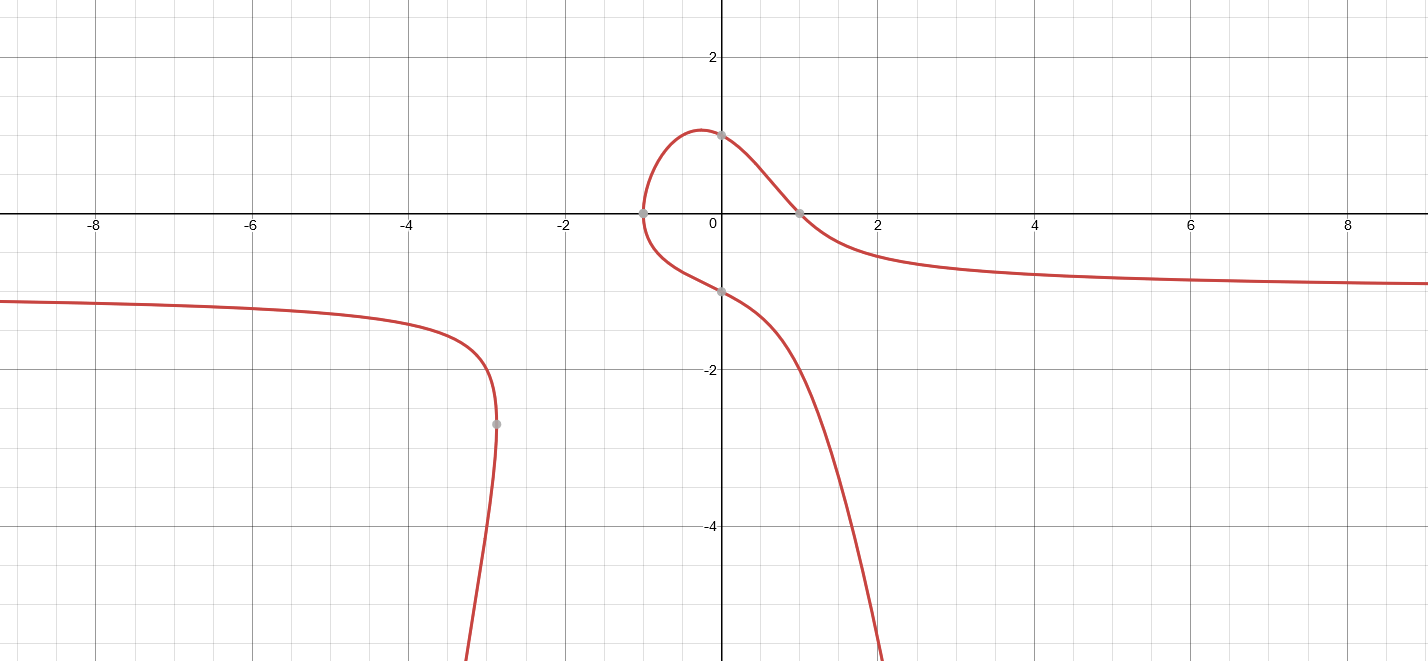
\includegraphics[width=\textwidth]{fig/Implicit2.PNG}
\index{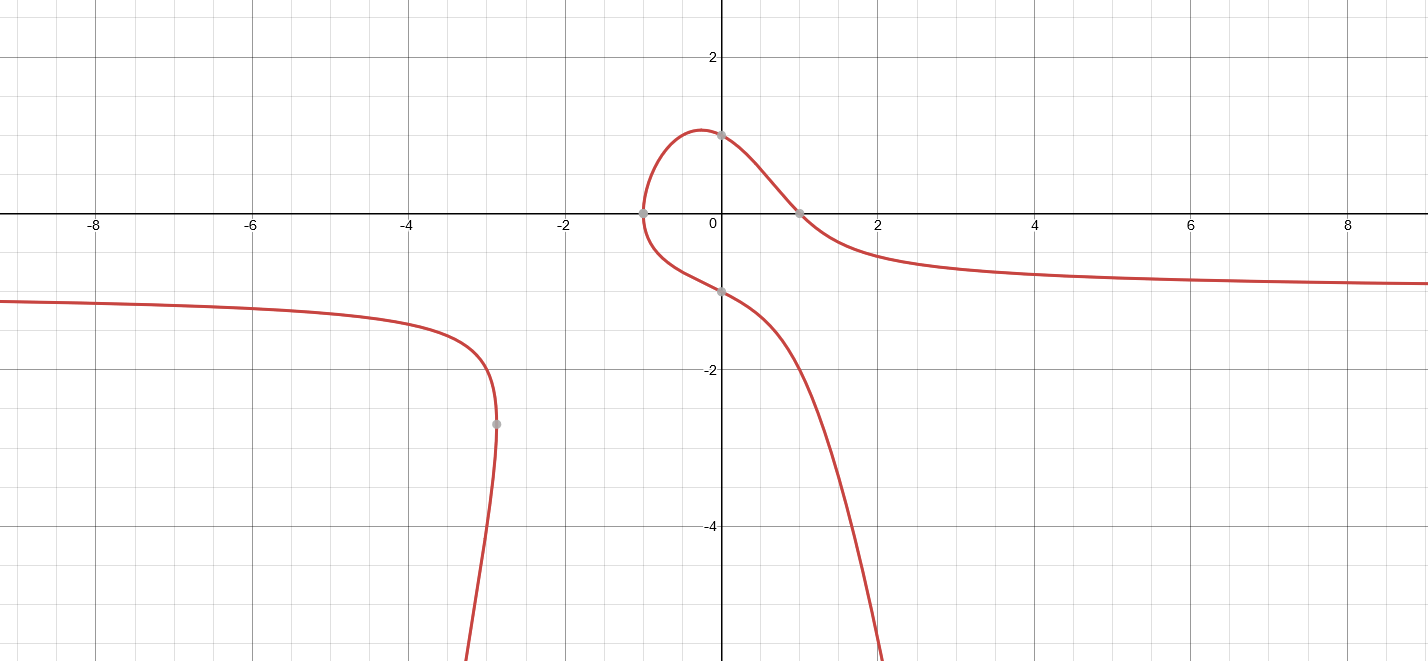
\includegraphics[height=5mm]{fig/Implicit2.PNG}screenshot of graph using Desmos Graphing Calculator, \url{https://www.desmos.com/calculator} (accessed 19 October 2017)}
\pause

Still has a slope: $\frac{\Delta y}{\Delta x}$ \pause \\
\textbf{Locally}, $y$ is still a function of $x$.
\end{frame}
%----------------------------------------------------------------------------------------
\begin{frame}[t]
\[y^2+x^2+xy+x^2y=1\]
 Consider $y$ as a function of $x$. Can we find $\diff{y}{x}$?
 
 \hfill  $\diff{}{x}[y]=$\pause\answer{$\diff{y}{x}=y'$}
 \hfill \pause
   $\diff{}{x}[x]= $\pause \answer{$1$}\hfill\pause
   $\diff{}{x}[1]=$ \pause \answer{$0$}
 \hfill~\pause
 \only<1-6>{\AnswerYes}\vfill
 
\iftoggle{printsolutions}{
	\color{answercolor}\small
	Differentiate both sides with respect to $x$.
	\begin{align*}
0&=2y\diff{y}{x}+2x+\left(x\diff{y}{x}+(1)y\right)+\left(x^2\diff{y}{x}+2xy\right)\\
0&=\diff{y}{x}\left(2y+x+x^2\right)+\left(2x+y+2xy\right)\\
-\left(2x+y+2xy\right)&=\diff{y}{x}\left(2y+x+x^2\right)\\
-\frac{2x+y+2xy}{2y+x+x^2}&=\diff{y}{x}
\end{align*}}{}
\end{frame}
%----------------------------------------------------------------------------------------
\begin{frame}[t]
\vspace{-5mm}
\[y^2+x^2+xy+x^2y=1\]

\[\diff{y}{x}=-\frac{2x+y+2xy}{2y+x+x^2}\]\pause

\only<-5>{Necessarily, $\diff{y}{x}$ depends on \textbf{both} $y$ and $x$. Why?}

\only<2,6>{\begin{center}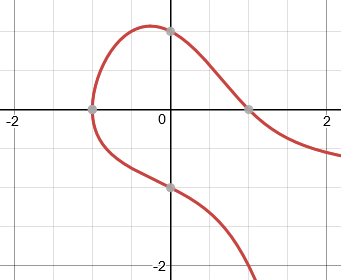
\includegraphics[width=4.5cm]{fig/Implicit.PNG}\pause\end{center}
\index{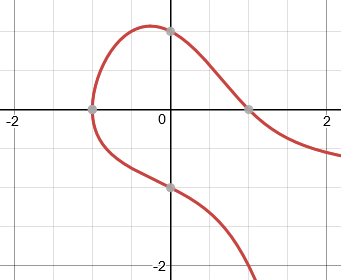
\includegraphics[height=5mm]{fig/Implicit.PNG} screenshot of graph using Desmos Graphing Calculator,  \url{https://www.desmos.com/calculator} (accessed 19 October 2017)}
}

\only<-5>{\answer{
\onslide<3->{\small
\begin{align*}
\left.\diff{y}{x}\right|_{\rlap{\tiny (1,0)}}&=\onslide<4->{\color{answercolor} - \frac{2(1)+0+2(1)(0)}{2(0)+1+1}}
&
\left.\diff{y}{x}\right|_{\rlap{\tiny (1,-2)}}&=\onslide<4->{\color{answercolor} -\frac{2(1)-2+2(1)(-2)}{2(-2)+1+1}}
\\
\onslide<4->{ &\color{answercolor}=-\frac{2}{2}=-1 & &\color{answercolor}=-2}
\end{align*}
}}}
\answer{
\onslide<5->{
\color{answercolor}  Points with the same $x$-value may have different slopes. We need both the $x$-value and the $y$-value to figure out which point we're talking about.}
}
\only<-3>{\AnswerYes}
\end{frame}
%----------------------------------------------------------------------------------------
\begin{frame}[t]
\only<1>{\AnswerYes
\QuestionBar{1}{2}}
\only<2>{\AnswerBar{1}{2}}

\NowYou Suppose $x^4y+y^4x=2$. Find $\diff{y}{x}$ at the point $(1,1)$.
\vfill

\note<2>{Students often struggle knowing when to replace variables with constants.}
\onslide<2|handout:0>{
\color{answercolor}
 \begin{align*}
x^4y(x)+y(x)^4x&=2\\
4x^3y(x)+x^4\diff{y}{x}(x)+y(x)^4+4y(x)^3\diff{y}{x}(x)\,x&=0
\intertext{We may only replace variables with constants \textit{after} differentiating. When $x=1$ and $y(1)=1$,}
4(1)^3y(1)+(1)^4\diff{y}{x}(1)+y(1)^4+4y(1)^3\diff{y}{x}(1)&=0\\
4+\diff{y}{x}(1)+1+4\diff{y}{x}(1)&=0\\
5\diff{y}{x}(1)&=-5\\
\diff{y}{x}(1)&=-1
\end{align*}
}

\end{frame}

%----------------------------------------------------------------------------------------
\begin{frame}<handout:0>
\note{It's nice to see what these things look like, but remind students we did NOT need this picture to solve the problem. (Otherwise, they may feel worried because they don't know how to graph these functions.)}
\AnswerBar{1}{2}
\color{answercolor}
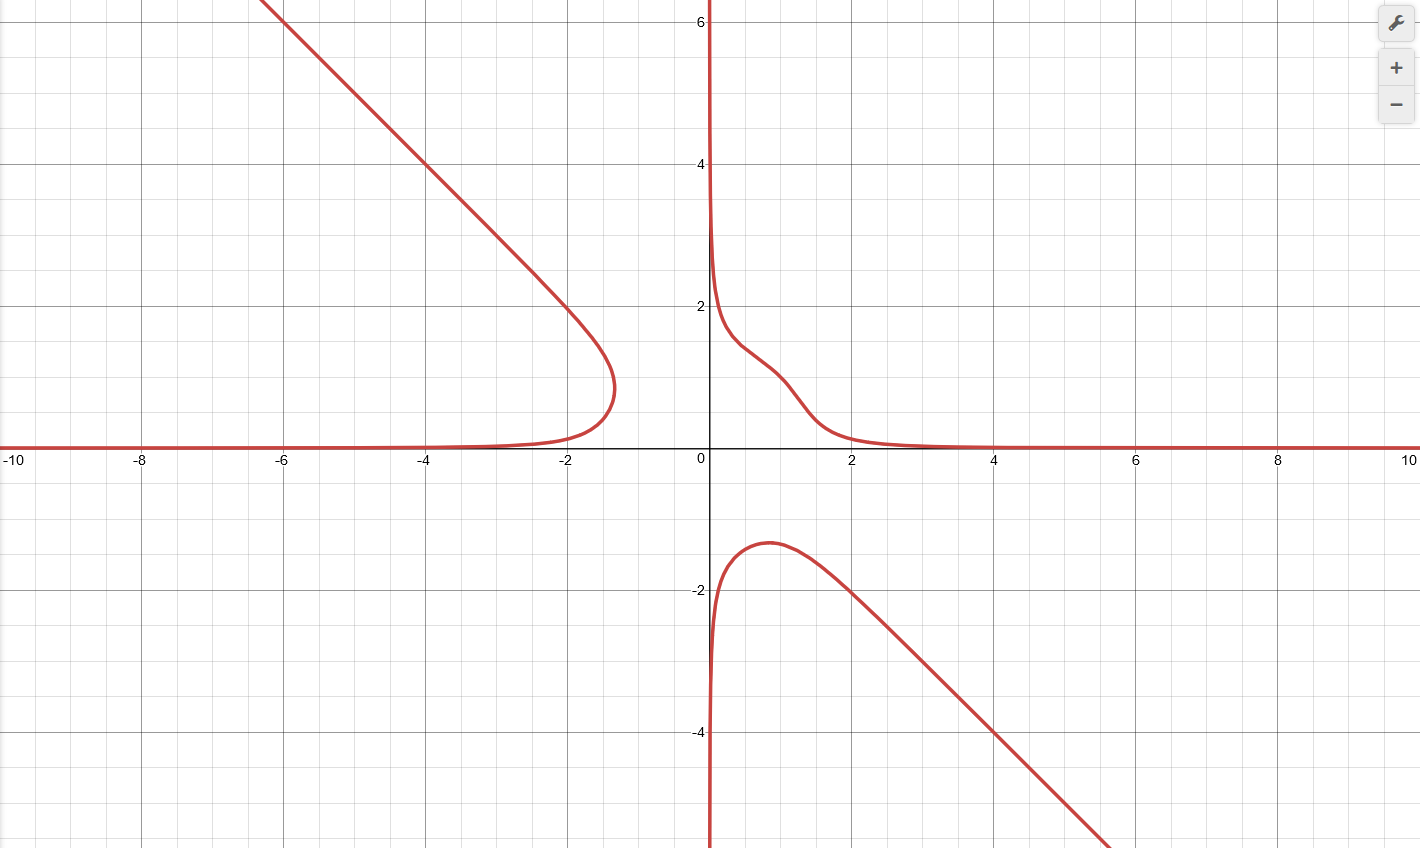
\includegraphics[width=\textwidth]{fig/Implicit3.png}\\
\index{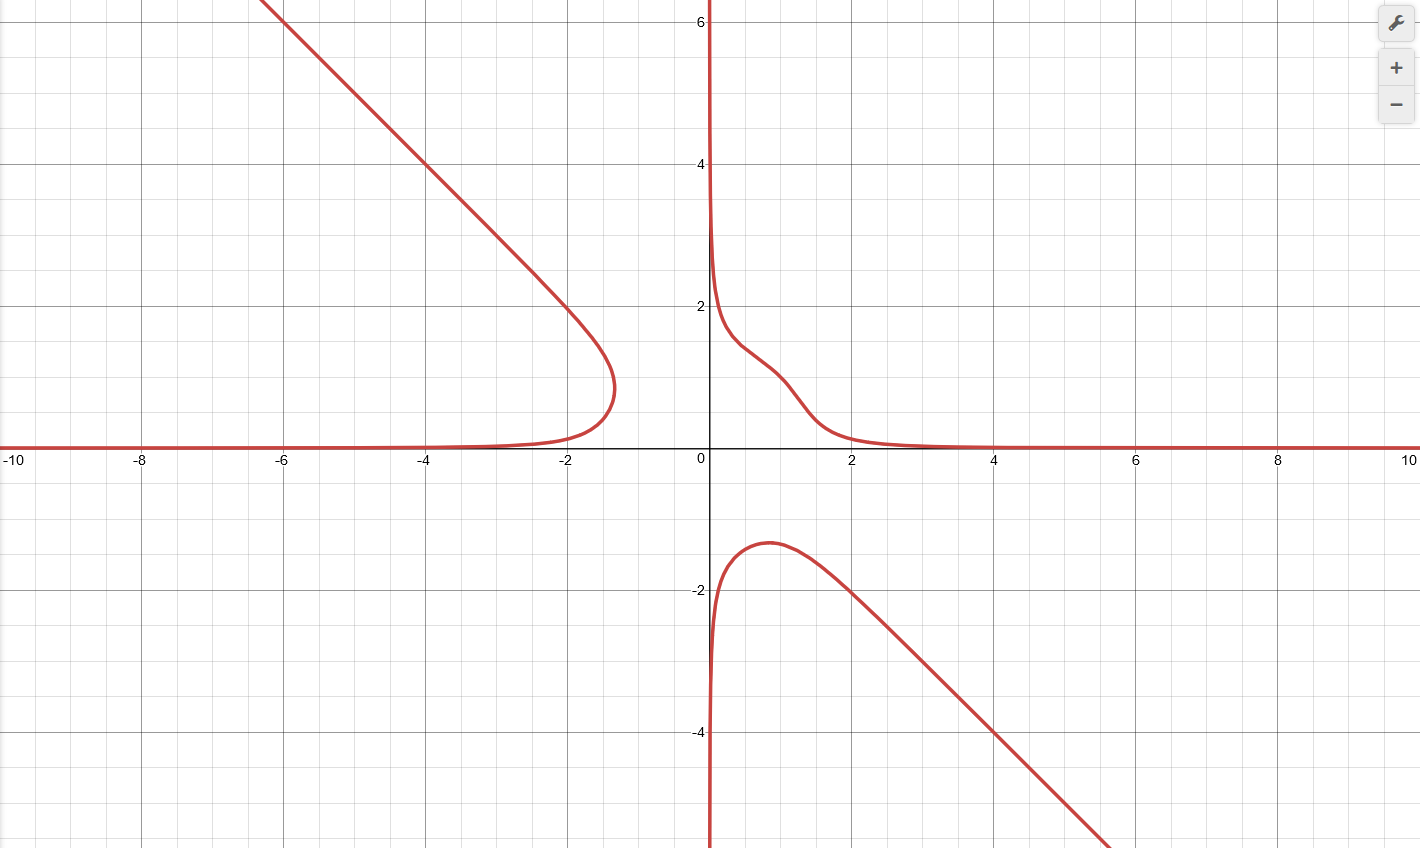
\includegraphics[height=5mm]{fig/Implicit3.png} screenshot of graph  using  Desmos Graphing Calculator, \url{https://www.desmos.com/calculator} (accessed 24 October 2018)}
\[x^4y+y^4x=2 \]
\end{frame}
%----------------------------------------------------------------------------------------
\begin{frame}[t]
\only<1>{\QuestionBar{2}{2}\AnswerYes}
\only<2>{\AnswerBar{2}{2}}
\NowYou Suppose $\dfrac{3y^2+2y+y^3}{x^2+1}=x$. Find $\ds\diff{y}{x}$ when $x=0$, and the equations of the associated tangent line(s).

\vfill
\onslide<2|handout:0>{
\color{answercolor}
	
To avoid the quotient rule, we start by simplifying our expression. 
\begin{align*}
\dfrac{3y(x)^2+2y(x)+y(x)^3}{x^2+1}&=x\\
3y(x)^2+2y(x)+y(x)^3&=x^3+x\\
6y(x)\diff{y}{x}(x)+2\diff{y}{x}(x)+3y(x)^2\diff{y}{x}(x)&=3x^2+1
\intertext{When $x=0$:}
\diff{y}{x}(0)&=\frac{1}{6y(0)+2+3y(0)^2 }
\end{align*}}
\end{frame}
%----------------------------------------------------------------------------------------

%%----------------------------------------------------------------------------------------
\begin{frame}<handout:0>
\color{answercolor}\AnswerBar{2}{2}
We need to know $y$ to find $\diff{y}{x}$. We want all points where $x=0$.
\begin{align*}
3y(0)^2+2y(0)+y(0)^3&=0\\
y(0)\big(y(0)^2+3y(0)+2\big)&=0\\
y(0)\big(y(0)+1\big)\big(y(0)+2\big)&=0\\
y(0)=0,\ y(0)=-1,\ y(0)&=-2
\end{align*}
\end{frame}
%%----------------------------------------------------------------------------------------
\begin{frame}<handout:0>
\color{answercolor}\AnswerBar{2}{2}
\[\diff{y}{x}=\frac{1}{6y+2+3y^2} \]
\begin{multicols}{3}
	$(0,0)$\\[10pt]
	$\left.\diff{y}{x}\right|_{(0,0)}=\frac{1}{2}$\\
	$y-0=\frac12(x-0)$\\
	$y=\frac12x$
	\columnbreak
	
	$(0,-1)$\\[10pt]
	\begin{align*}\textstyle
          \left.\diff{y}{x}\right|_{(0,-1)}&=\textstyle\frac{1}{-6+2+3}\\
                        &=-1\end{align*}\\
         $y-(-1)=-1(x-0)$\\
         $y=-x-1$
	
	\columnbreak
	$(0,-2)$\\[10pt]
	\begin{align*}\textstyle\left.\diff{y}{x}\right|_{(0,-2)}
                           &=\textstyle\frac{1}{-12+2+12}\\
                           &=\textstyle\frac12\end{align*}\\
$y-(-2)=\frac12(x-0)$\\
$y=\frac12x-2$
	\end{multicols}
\end{frame}
%%----------------------------------------------------------------------------------------

	\begin{frame}<handout:0>
	\AnswerBar{2}{2}
	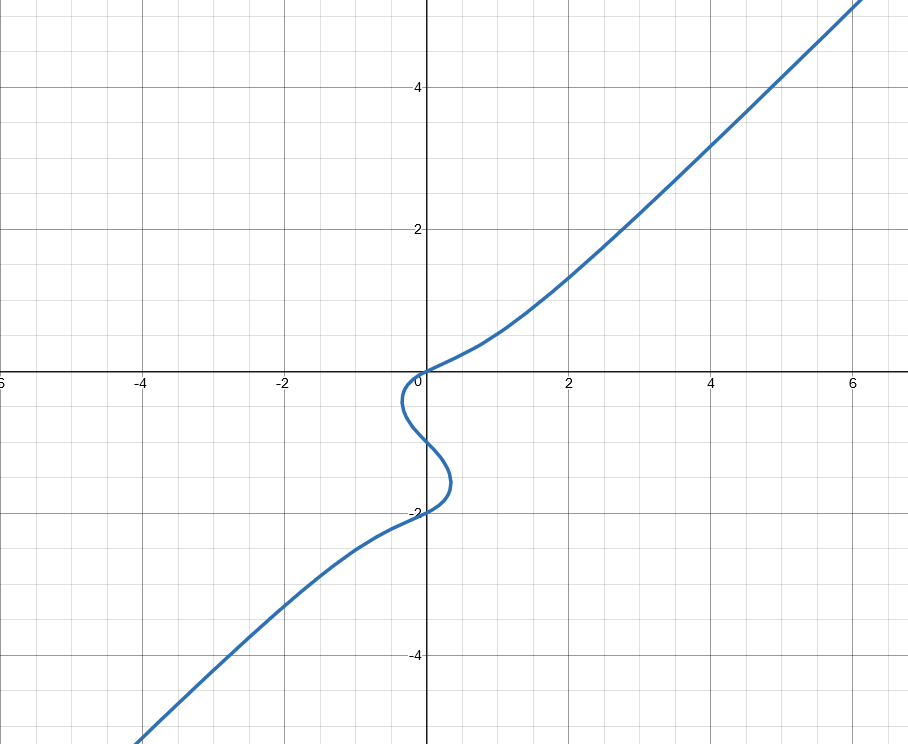
\includegraphics[width=.75\textwidth]{fig/Implicit4.png}\\
	\index{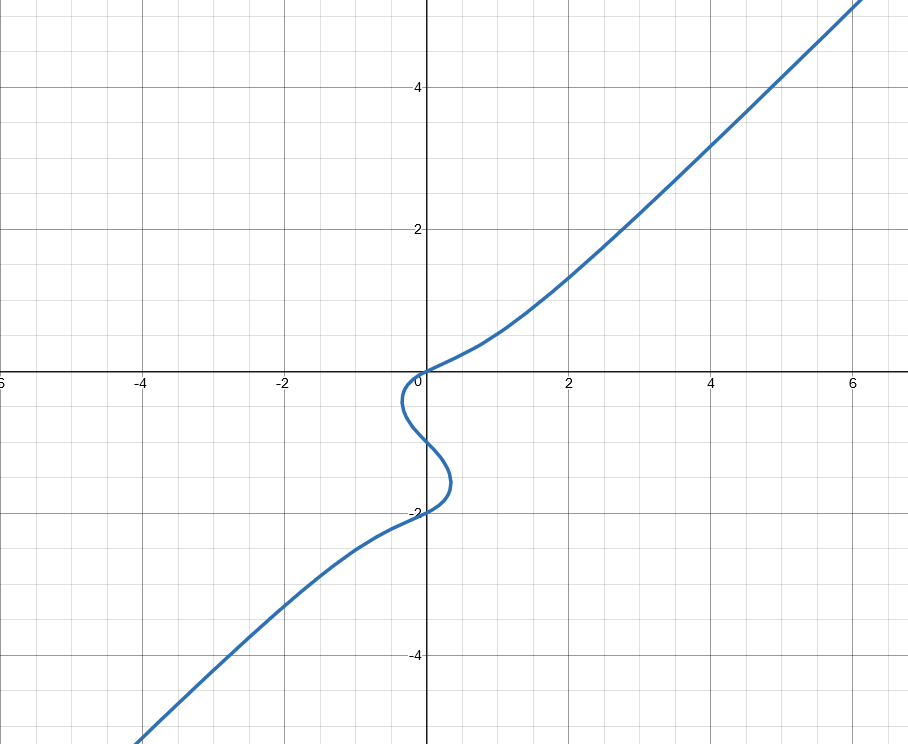
\includegraphics[height=5mm]{fig/Implicit4.png}  screenshot of graph   using Desmos Graphing Calculator,  \url{https://www.desmos.com/calculator}, (accessed 24 October 2018)}
	\[\dfrac{3y^2+2y+y^3}{x^2+1}=x\]
\end{frame}

%----------------------------------------------------------------------------------------
\begin{frame}<handout:0>
\AnswerBar{2}{2}
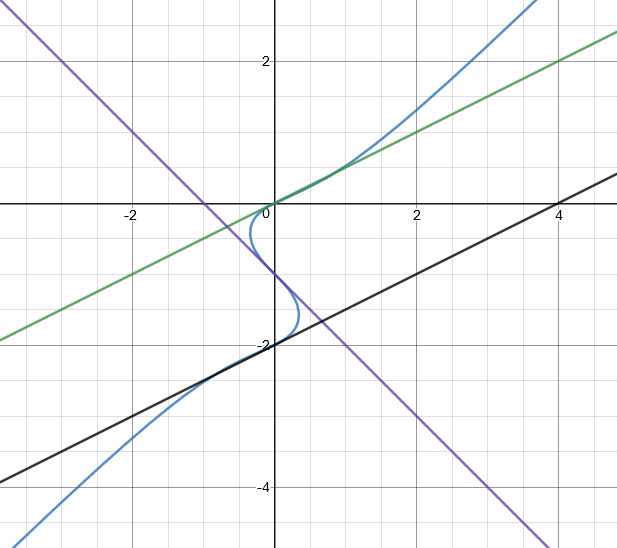
\includegraphics[width=.7\textwidth]{fig/Implicit6.png}\\
\index{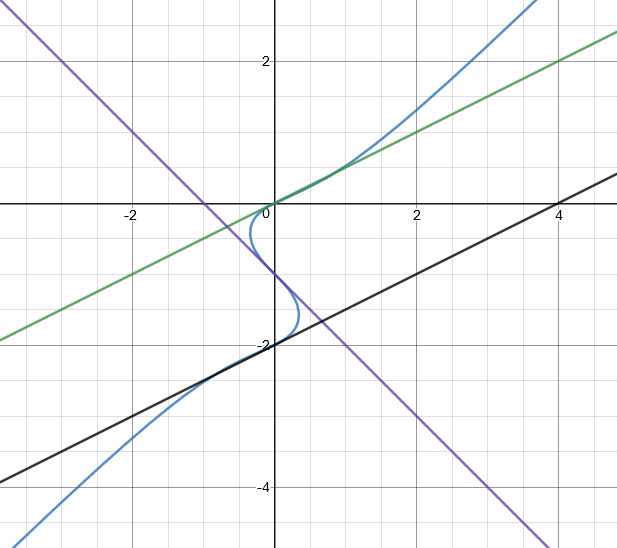
\includegraphics[height=5mm]{fig/Implicit6.png}  screenshot of graph   using  Desmos Graphing Calculator, \url{https://www.desmos.com/calculator} (accessed 24 October 2018)}
\[\dfrac{3y^2+2y+y^3}{x^2+1}=x\]
\end{frame}


%----------------------------------------------------------------------------------------
%------------------------------------------------------------------
\begin{frame}[t]
\only<1-2>{\AnswerYes}
Use implicit differentiation to differentiate $\log(x)$, $x>0$.\color{answercolor}
\only<2-4>{\begin{align*}
\log x &= y(x)\\
x&=e^{y(x)}\\
\onslide<3-|handout:0>{
1&=e^{y(x)} \cdot \diff{y}{x}(x)\\
\diff{y}{x}(x)&=\frac1{e^{y(x)}}=\frac1x
}
\end{align*}}\vfill

\onslide<4->{\textcolor{black}{Use implicit differentiation to differentiate $\log|x|$, $x<0$.}}
\only<4>{\AnswerYes\MoreSpace}
\onslide<6-|handout:0>{
\begin{align*}
\log |x| &= y(x)\\
\log(-x)&=y(x)\\
-x&=e^{y(x)}\\
-1=e^{y(x)}\cdot\diff{y}{x}(x)\\
\diff{y}{x}(x)&=\frac{-1}{e^{y(x)}}=\frac{-1}{-x}=\frac1x
\end{align*}
}
\end{frame}
%----------------------------------------------------------------------------------------
\begin{frame}[t]
Use implicit differentiation to differentiate $\log_a(x)$, where $a>0$ is a constant and $x>0$.
\vfill
Use implicit differentiation to differentiate $\log_a|x|$, $a>0$.
\vfill
\AnswerYes\MoreSpace
\end{frame}
%------------------------------------------------------------------
\begin{frame}<handout:0>[t]
Use implicit differentiation to differentiate $\log_a(x)$, where $a>0$ is a constant and $x>0$.\pause
\color{answercolor}\vfill

\begin{align*}
\log_a x &= y(x)\\
x&=a^{y(x)}\\
1&=a^{y(x)} \cdot \log_e a \cdot \diff{y}{x}(x)\\
\diff{y}{x}(x)&=\frac{1}{a^{y(x)} \cdot \log_e a} = \frac{1}{x\log_e a}
\end{align*}


\end{frame}
%------------------------------------------------------------------
\begin{frame}<handout:0>[t]
Use implicit differentiation to differentiate $\log_a|x|$, $a>0$.\pause
\color{answercolor}\vfill

If $x>0$, it's what we just computed. So assume $x<0$.

\begin{align*}
\log_a |x| &= y(x)\\
\log_a (-x) &= y(x)\\
-x&=a^{y(x)}\\
-1&=a^{y(x)} \cdot \log_e a \cdot \diff{y}{x}(x)\\
\diff{y}{x}(x)&=\frac{-1}{a^{y(x)} \cdot \log_e a} = \frac{-1}{x\log_e a}
\end{align*}

\end{frame}
%----------------------------------------------------------------------------------------
%----------------------------------------------------------------------------------------

